
% document settings
%%%%%%%%%%%%%%%%%%%%%%%%%%%%%%%%%%%%
\documentclass[final,3p,times,authoryear,12pt]{elsarticle}

\usepackage{amsfonts}
\usepackage{mathtools}
\usepackage{cancel}
\usepackage{amsthm}
\usepackage{amsmath}
\usepackage{amssymb}
\usepackage{dsfont}
\usepackage[dvipsnames,usenames]{color}
\usepackage[colorlinks=true,linkcolor=NavyBlue,citecolor=NavyBlue,urlcolor=NavyBlue]{hyperref} % for hyperlinks 
\usepackage{floatpag}
\usepackage{hyperref}
\usepackage[shortlabels]{enumitem} 

% macros 
%%%%%%%%%%%%%%%%%%%%%%%%%%%%%%%%%%%%%%%%%%%%%%%%%%%%%%%%%%%%%%%%%%%%%%%%%%%%
\newcommand{\R}{\mathds {R}}
\newcommand{\red}[1]{\textcolor{WildStrawberry}{#1}} % for color for remarks
\newcommand{\green}[1]{\textcolor{Green}{#1}} % for color for remarks

% remove abstracf (for now)
%%%%%%%%%%%%%%%%%%%%%%%%%%%%%%%%%%%%%%%%%%%%%%%%%%%%%%%%%%%%%%%%%%%%%%%%%%%%
\makeatletter
\long\def\MaketitleBox{%
  \resetTitleCounters
  \def\baselinestretch{1}%
  \begin{center}%
   \def\baselinestretch{1}%
    \Large\@title\par\vskip18pt
    \normalsize\elsauthors\par\vskip10pt
    \footnotesize\itshape\elsaddress\par\vskip36pt
%    \hrule\vskip12pt
%    \ifvoid\absbox\else\unvbox\absbox\par\vskip10pt\fi
%    \ifvoid\keybox\else\unvbox\keybox\par\vskip10pt\fi
%    \hrule\vskip12pt
    \end{center}%
  }
\makeatother

% title, authors and affiliations
%%%%%%%%%%%%%%%%%%%%%%%%%%%%%%%%%%%%
\journal{~}
\begin{document}
\begin{frontmatter}

\title{Fair, Stable Exchange Networks through Quenched Merchant Location and Idiosyncratic Trading Costs}

\author[add1]{Nate Dwyer}
\ead{nate9799@gmail.com}

\author[add1]{Sandro Claudio Lera}
\ead{slera@mit.edu}

\author[add1]{Alex `Sandy' Pentland}
\ead{sandy@media.mit.edu}

\address[add1]{\scriptsize The Media Lab, Massachusetts Institute of Technology, 77 Massachusetts Avenue, 02139 Cambridge, Massachusetts, USA}

%%%%%%%%%%%%%%%%%%%%%%%%%%%%%%%%%%%%
\begin{abstract} 
A new, firm-buyer specific idiosyncratic tax is introduced.
\end{abstract}

\end{frontmatter}
%%%%%%%%%%%%%%%%%%%%%%%%%%%%%%%%%%%%


\section{Introduction}
%%%%%%%%%%%%%%%%%%%%%%%%%%%%%%%%%%%%%%%%%%%%%%%%%%%%%%%%%%%%%%%%%%%%%%%%%%%%

Until not too long ago, people used to live in more self-contained villages,
with local markets where people buy different products.  Take clothing as an
example. Most villages had one or more clothing merchants competing for
customers.  There is some healthy competition among merchants within a village,
as people can flexibly switch according to prices and preferences. But customers
would rarely buy clothing from a faraway village, as the transaction cost
associated with visiting that village would be high,  and could not offset a
marginally better price or quality.  On the other hand, people living far away
from any village were disadvantaged as they would always incur such high costs.
Similarly, if there is a specialized product that can only be produced in some
villages, it was harder to find customers across village borders, making it more
difficult for new products and technologies to succeed. 

From the industrial to the technological revolution, more efficient distribution
channels have emerged, enabling people to buy almost any product in online
stores. Now, orders can be delivered to their door within a day independent of a
customer's physical location  More specialized products are now sold globally,
and even people living far away from cities benefit from the availability of a
wide range of products. While such efficiency is beneficial for the economy as a
whole, it comes at the cost of potential monopolies.  Consider a merchant that
manages to sell a product for a few cents cheaper than its competitors.  Given
modern distribution channels, and ignoring potential differences in quality,
every buyer is now incentivized to buy from that one firm offering the cheaper
price. One potential outcome is that the competitors follow along, increase
their efficiency, and a new equilibrium is reached.  However, in a suboptimal
scenario, that one firm leverages the temporarily increased revenue to further
outpace and potentially undercut its competitors.  In the short term, feedback
mechanisms kick in, and an initially minor gap in competitive advantage, mixed
with efficient distribution channels, manifests itself in a suboptimal monopoly. 

In this article, we show that such monopolies can be prevented by introducing an idiosyncratic buyer-seller transaction cost.
This tax leverages the benefits of modern distribution channels, making sure that no buyer remains disadvantaged. 
At the same time, innovative products can spread globally, whereas less specialized products remain local. 
This is achieved through the following taxation mechanism: 
Consider a set of $|F|$ firms, all offering the same product, and a set of $|B|$ potential buyers (customers). 
For any buyer $b \in B$ and firm $f \in F$, we define the ordinal distance $D = D(b,f)$ such that the firm $f$ that is physically closest to $b$ has distance $D(b,f)=1$, the next closest has distance $D=2$, and the $n$-th closest has distance $D=n$. 
The tax when customer $b$ buys from the $n$-th closest firm is then proportional to $D^\gamma$, for some exponent $\gamma > 0$. 
If we were to set $\gamma = 0$, everybody can buy from every firm at the same tax rate. 
If we were to set $\gamma=\infty$, a seller can only buy from its closest firm.
A gamma in-between those two extremes represents a trade-off: 
Close-by products are taxed less than far away products. 
However, because the distance is ordinal, absolute distances do not matter. 
No matter whether the next closest firm is $100$ meters or $100$ kilometres, the taxation is the same. 
In particular, if there is only one firm offering the product, everybody buys for the same tax (since $D=1$ for every buyer), enabling innovations to spread globally.  

Through tuning of $\gamma$ and targeted redistribution of tax money to regions of low economic activity, we show that this model is able to fuel a self-consistent economy, 
with fair competition, where innovations can spread freely, but without the chance of monopolies emerging through disproportional feedback mechanisms. 
In summary, we present a model that avoids the winner-take-all monopoly tendency and associated negative externalities of today's Internet enabled business through a discretised, distance-based tax. 

\section{Model Set-Up}
%%%%%%%%%%%%%%%%%%%%%%%%%%%%%%%%%%%%%%%%%%%%%%%%%%%%%%%%%%%%%%%%%%%%%%%%%%%%

We simulate an economy of firms and customers in some environment with a distance metric (e.g. a country using road distance) and study how firms respond to the idiosyncratic tax.
In this section, we outline the model semi-quantitatively. 
Game-theoretical details are then elaborated in section \ref{sec:game_theory} and concrete applications are described in the subsequent sections. 
Section \ref{sec:conclusions} summarises the results and suggests future directions. 

\subsection{Geography}
The geography of our model is one-dimensional with periodic boundaries (i.e. a topological circle) of length $L$. 
Due to the periodic boundary conditions, we measure physical distances with the metric $\min(|b-f|, L-|b-f|)$ for any two points $b$,$f$ (i.e. buyers and firms) on the circle. 
Without loss of generality, we set $L=1$. 
The left-hand-side plots of Figure \ref{fig:static_game} are examples of this `abstract geography'.
Our results not rely on the implemented geography, and any other, potentially more realistic topology could be considered.
However, as we outline above, a simple ring-topology is sufficient for practical purposes, and could be implemented on digital market places such as Amazon. 

\subsection{Product}
In a first approach, we consider an economy of only one product. 
We assume that all firms produce that same product, but at potentially different production costs. 
Extensions to more products are essentially straight forward and discussed in the outlook section below. 

\subsection{Buyers}
Buyers are placed on the circle uniformly at random. 
Each buyer tries to buy as much product as possible, but is constrained by a negatively sloped demand curve which lowers the amount of product they can buy the more expensive the product gets.

\subsection{Firms}
The firms, like the buyers, are also randomly placed on the circle, and compete non-cooperatively to maximize their profit. 
In this competition, also known as a `game' in the context of game theory, each firm makes two choices, first capacity (i.e. how much they produce), then price. 
A firm chooses capacity before price because it is difficult to adapt capacity due to supply chain restraints, while it is easier to change a price tag.

For the remainder of this article, the location of buyers and sellers is held fixed. 
This can be relaxed later on, assuming that their location changes on time-scales slower than numerous transactions with clients. 

\subsection{Idiosyncratic Tax}
The idiosyncratic tax that is introduced by this paper is dependent on a distance measure $D$, or ordinal distance, that gives a discrete distance between every pair of buyers and firms. 
We define the ordinal distance $D$ be defined such that the closest firm to a buyer is at ordinal distance $D=1$, the next closest at $D=2$, and the $n$th closest at $D=n$. 
If buyer $b$ wants to buy a product from its $n$-th closest firms, a tax proportional to $n^\gamma$ for some $\gamma \geqslant 0$ is raised. 
This incentivizes buyers to purchase from more local firms, unless a remote firm offers the same product for a considerably lower price, offsetting the tax. 

Crucially, this ordinal distance is calculated for every individual type of product. 
For instance, a car manufacturer and a bakery do not increase each other's distance from their buyers.
Thus, if a firm produces a new product, such as a drug for a previously incurable disease, it is considered at distance $D=1$ from all buyers, at least until a competitor emerges.
This way, new technologies and true innovation can spread freely, whereas more basic products remain more localized. 

\section{Equilibrium Capacities \& Prices}
\label{sec:game_theory} 
%%%%%%%%%%%%%%%%%%%%%%%%%%%%%%%%%%%%%%%%%%%%%%%%%%%%%%%%%%%%%%%%%%%%%%%%%%%%

In this section, we explain how firms set their production quantities and prices based on game theoretic equilibria. 
The reader only interested in qualitative results may skip this section and continue reading in section \ref{sec:static_game}. 

When firms choose capacity and price, they make their choices in order to maximize profit. 
First, the firms compete on capacity, by simultaneously declaring how much of the product they plan to produce; next, they compete on price to determine the firms' non-tax prices. 
This process, consisting of these two sub-games, is similar to the games studied by \cite{kreps1983quantity}.
From a game-theoretical perspective, the major difference is the idiosyncratic tax, which significantly alters the pricing sub-game.

The exact quantity and price offered by each firm are determined as the Nash equilibrium of this two-stage game. 
The firm's strategy-space is thus given by the number of quantity that they produce and the prices that they can offer. 

\subsection{Capacity Game}
The first choice is how much capacity $\hat q_f$ each firm $f$ wishes to produce.
The firm's desire to increase capacity is limited by two factors.
First, firm $f$ incurs a unit price of $c_f$ for every unit of product they
install, regardless of whether or not the product is sold. 
Second, buyers have limited demand. 

%put the '\footnote' right next to the period to avoid weird spacing between footnote and end of sentence
The capacity sub-game acts much like a Cournot game.\footnote{
A Cournot game is where firms compete only on quantity, and sell all of the quantity at the market clearing price.} 
The difference is that instead of firms being assigned a
market clearing price and selling everything they produce, in our model the
firms compete on price in a second sub-game where they choose a price. This
sub-game is necessary because the idiosyncratic tax can provide incentive for
firms to charge different prices. For example, a firm with low costs trying to
sell to non-local buyers would need to undercut firms that are more local to those potential customers. 
Depending on the tax, this may or may not increase profits. 

\subsection{Pricing Game}

Each firm $f$, having chosen a capacity $\hat q_f$, now chooses a price, $p_f$. 

By choosing a lower price, a firm can undercut competitors. 
Since the amount a buyer purchases increases as the product gets less expensive, a lower price increases the amount of product purchased in total. 

Note that usually, it is not optimal for a firm to offer products so cheaply that it can sell to the entire market. 
It tends to be more profitable to sell a lower quantity locally at a higher price.\green{I don't know if I would go this far here.}

\subsection{Idiosyncratic Tax}
The idiosyncratic tax is designed to promote buyers purchasing locally by
imposing no tax if a buyer purchases from the nearest firm, and then increasing
the tax in discrete steps as firms get more and more ordinally distant. Since
each buyer-seller pair can have a different tax, the tax can cause two buyers
to perceive separate prices at the same firm.

\green{This is the third time we define ordinal distance. We should cut at least
one}
For any buyer $b$ and firm $f$, we define the ordinal distance $D = D(b,f)$
such that the firm $f$ that is physically closest to $b$ has distance
$D(b,f)=1$, the next closest has distance $D=2$, and the $n$th closest has
distance $D=n$.  Thus, if buyer $b$ buys from firm $f$, the total price,
including tax, is given by 
\begin{equation}
	p(b,f) = p_f + p_f ~ r~ \left( D(b,f)^\gamma - 1 \right)
\end{equation}
where $\gamma$ is the coefficient governing how quickly the tax increases, and
$r$ is a simple scaling coefficient (set to $100\%$ in the remainder of this
report\green{in teh bar plots, $r=1$}). 

Implementing this tax gives the buyers individualized preferences over the firms. 
For example, imagine two firms $f$ and $g$, and let $p_f <p_g$. 
Without any tax, every buyer prefers buying from $f$ versus buying from $g$. 
But with the tax, this could change. 
Say that buyer $b$ is very close to firm $g$, and very far from firm $f$ (in the sense that there is many other firms in-between). 
This implies $D(b,f) \gg D(b,g)$ and hence $p(b,f) > p(b,g)$, such that $b$ busy from $g$. 
Quantitative examples are provided in section \ref{sec:static_game}. 

There are two limit cases: $\gamma=0$ and $\gamma=\infty$. 
When $\gamma = 0$, no firms are taxed anywhere, so the game simplifies into a pure \cite{kreps1983quantity} game.
In contrast, when $\gamma = \infty$, it becomes impossible for buyers to purchase from non local firms, and so the firms all impose monopolistic prices.

\subsection{Buyer Allocation} 

Consider two vending machines right beside one another selling the same soda, with one machine selling soda at a cheaper price than the other. 
Customers will buy from the cheaper machine first until it runs out, and will then switch to the more expensive machine until their demand is satisfied. 
This generic type of consumer behaviour is implemented in our two-step game as well: 
buyer's start buying from the cheapest buyer first (incl. taxes), then move on to the second cheapest, and so forth. 
Throughout the game, we assume global information, i.e. buyers are perfectly aware of all prices. 
This is good approximation of reality when considering digital market places such as Amazon. 

More formally, let the set of buyers be called $B$. 
Each buyer $b\in B$ buys a quantity $q_b =\sum_{f\in F} q_{b,f}$, where $q_{b,f}$ is the amount buyer $b$ buys from the firm $f$. 
The buyers all have identical demand curves $p_\text{max} + q_b = a$, where $a$ is the endowment, and $p_\text{max}$ is the maximum price they buy product at (including tax). 
Each buyer tries to maximize $q_b$ while keeping $p_\text{max} + q_b \le a$. 
In other words, they buy from the cheapest available firm until they hit the demand curve and stop buying, or the firm runs out of capacity and the buyer begins buying from the next cheapest, repeating the process.

If a buyer perceives multiple firms as offering identical prices, they buy from
all such firms in identical amounts until either the buyer hits their demand
curve, or a seller runs out of capacity. 
This assumption is known as rationing. 

\subsection{Profit Function}
After having produced $\hat q_f$ units sold at price $p_f$, firm $f$'s profit is given by 
\begin{equation}
    \Pi_f = p_f \sum_{b\in B} q_{b,f} - c_f\hat q_f,
\end{equation} 
where  $p_f \sum_{b\in B} q_{b,f}$ is the firm's revenue, and $ c_f\hat q_f$ is the firm's total cost.
Taxes affect the firm's profit by altering buyer's preferences, hence changing $q_{b,f}$.

If the firm sells all of their capacity, then $q_f = \hat q_f$, and the profit equation simplifies to:
\begin{equation}
    \Pi_f = (p_f- c_f) \hat q_f,
\end{equation}
which is the net profit per unit multiplied by quantity sold.

\subsection{Numerical Solution of Nash Equilibria}

The firms choose their capacity and price such that they are in a Nash equilibrium. 
Because of the idiosyncratic structure of the game, which depends on the exact location of buyers and sellers, 
it is not possible to determine the Nash equilibrium analytically, for general cases. 
Instead, we use the Gambit library developed by  \cite{gambitPython} to find the Nash equilibrium numerically. 
To this end, the strategy space of capacities and prices are discretised into a sufficiently fine grid. 
Then, the quantity-price two-step game is solved in reverse order: 
For every choice of quantity, the equilibrium price is determined.
Then, the equilibrium quantity is determined. 
Example solutions are provided in the next section. 

\section{Towards a More Balanced Economy}
\label{sec:static_game}
%%%%%%%%%%%%%%%%%%%%%%%%%%%%%%%%%%%%%%%%%%%%%%%%%%%%%%%%%%%%%%%%%%%%%%%%%%%%

\begin{figure}[[p!htb] % p stands for 'entire page', '!htb' is to insert as close to code as possible
  \floatpagestyle{empty} % remove page number
  \centering
  \vspace{-2cm} % shift upwards to get more space for caption
  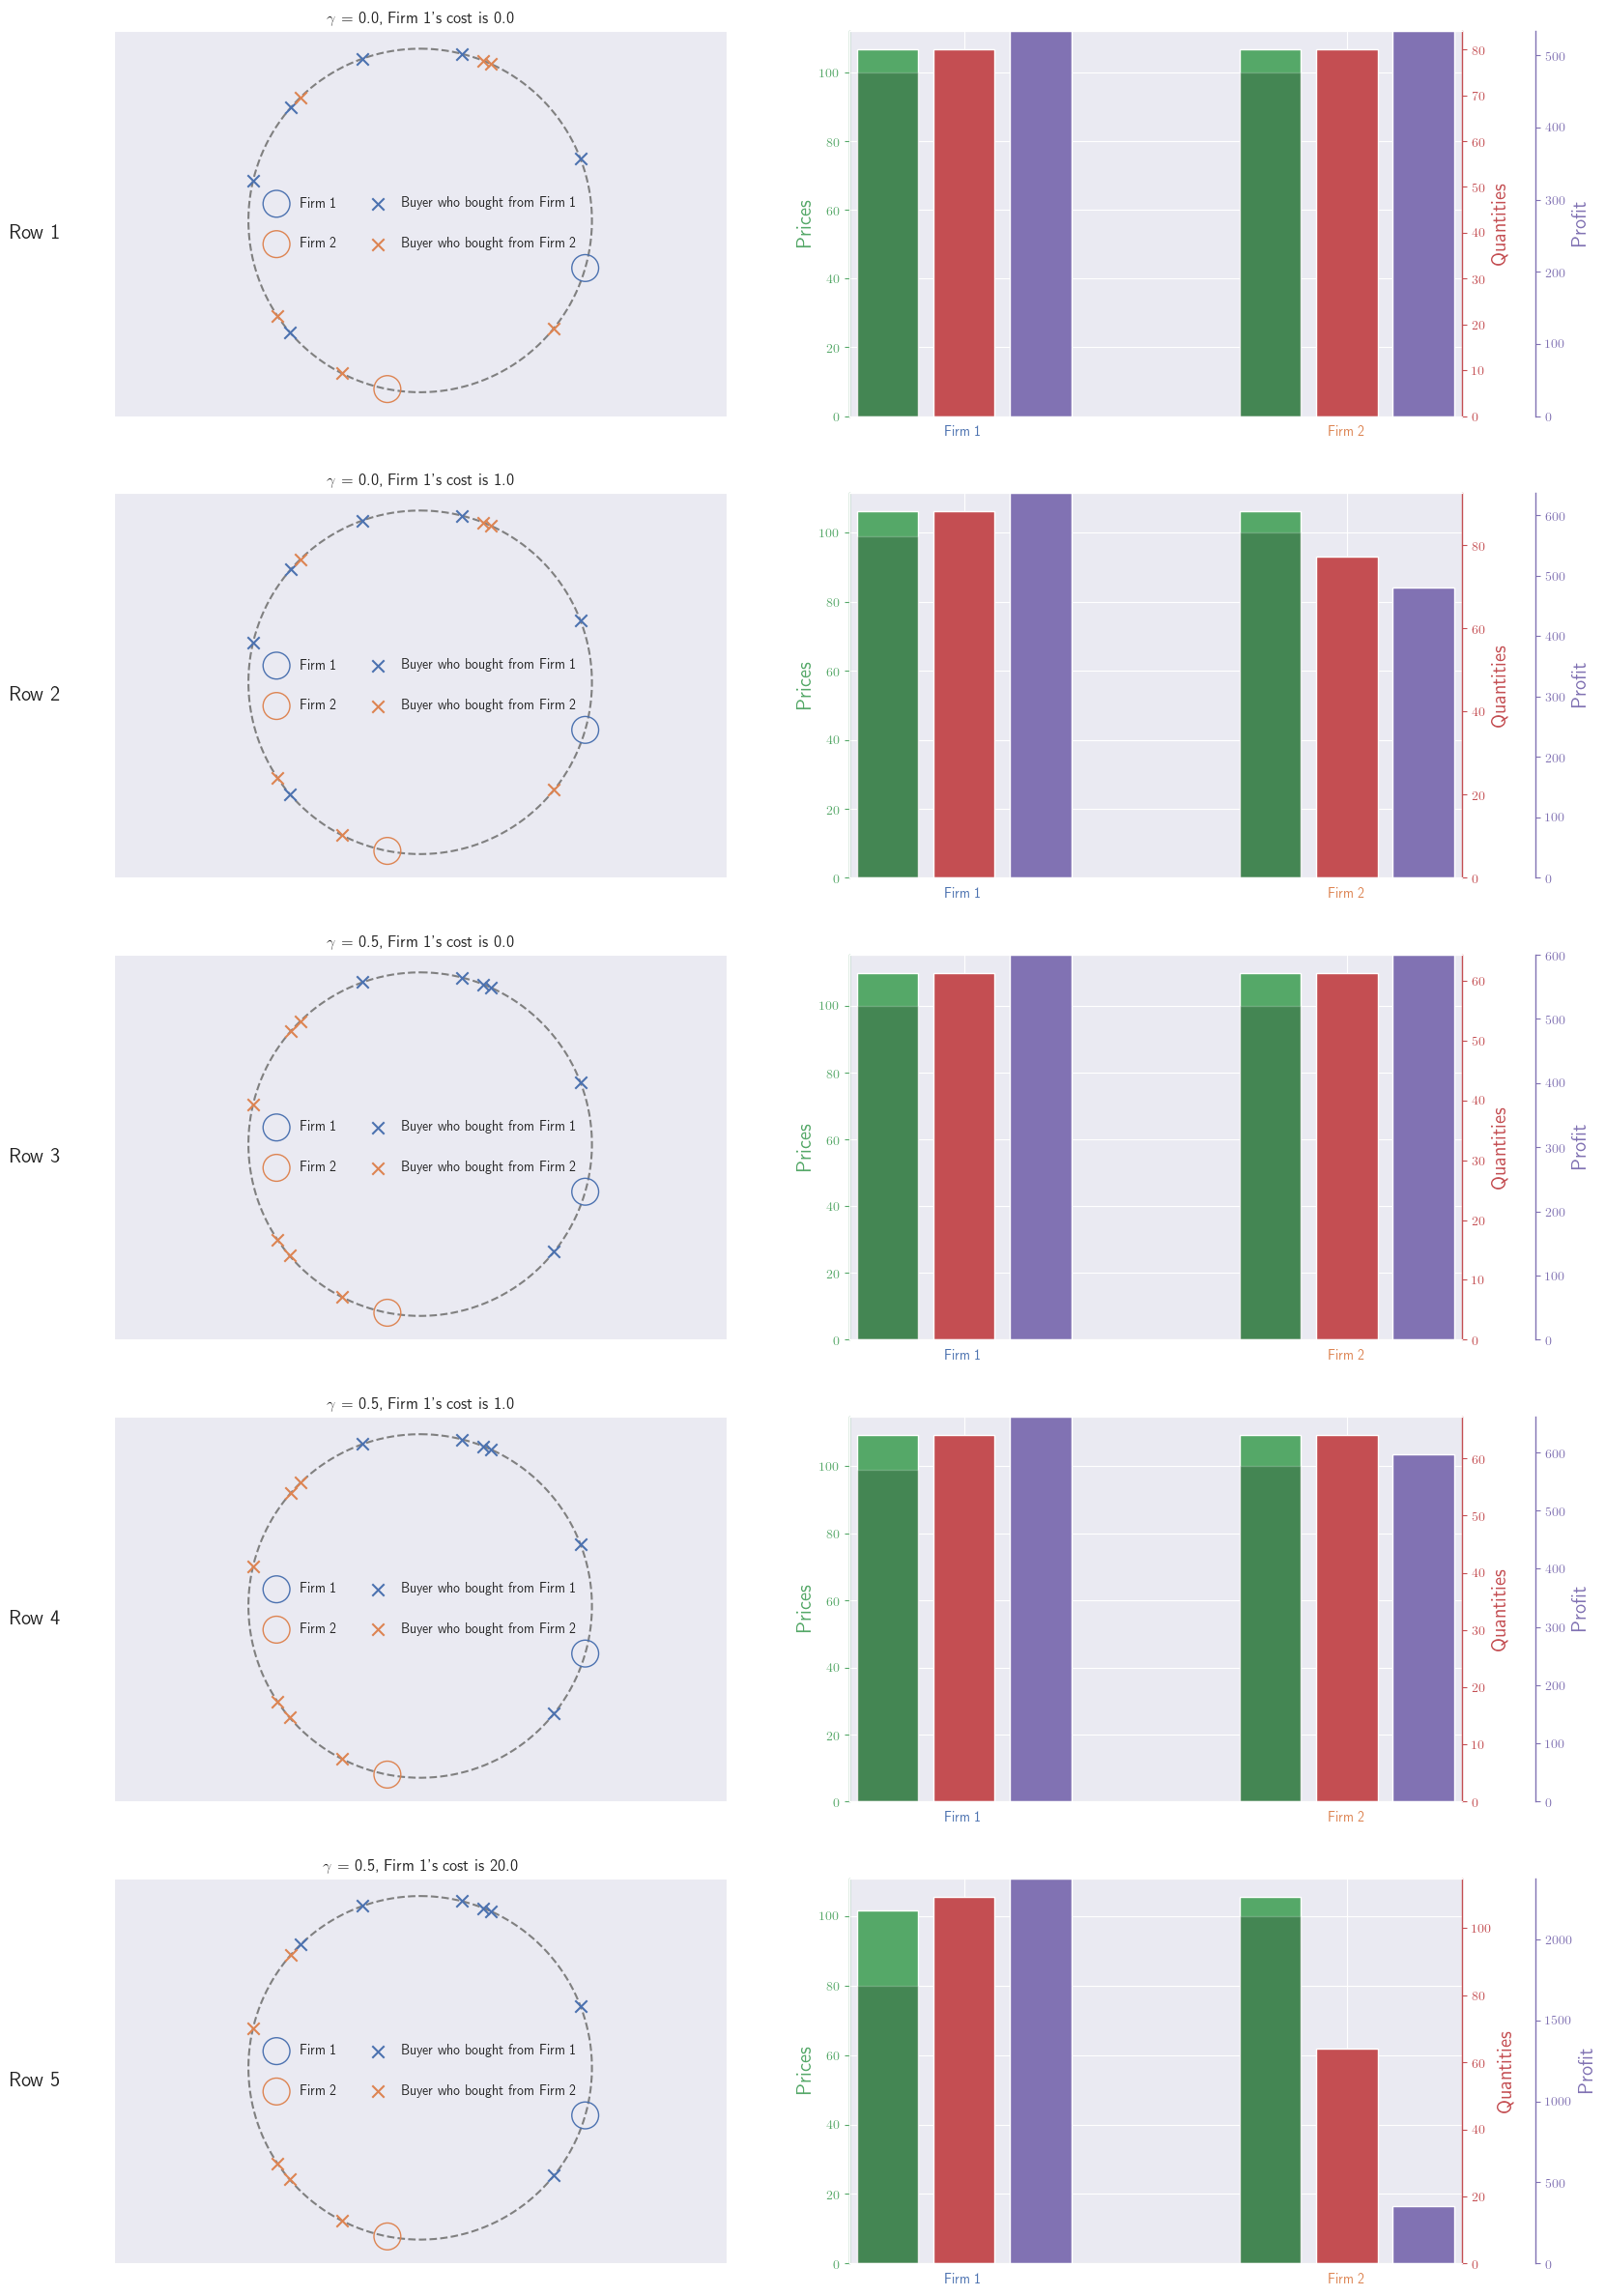
\includegraphics[width=\linewidth]{static_game.png}
  \caption{\small{
  		The balancing effect of the distance-based tax is demonstrated. 
		The first two rows depict an economy where the is no distance-based tax. 
		If costs are equal, the profits are equal as well. 
		But if costs are marginally different, the game-theoretical equilibrium profit are disproportionally large. 
		The mitigating effect of a distance-based tax is considered in rows 3-5. 
		If costs are equal (row 3) or marginally different (row 4), then profits are only marginally different. 
		But if costs are significantly different (row 5), so are the equilibrium profits. 
		An interpretation in an economic context is provided in the text of subsection \ref{sec:static_economy}. 
		 }}
  \label{fig:static_game}
\end{figure}

\subsection{A Static Economy} 
\label{sec:static_economy}

We are now demonstrating the social benefits of this taxation policy by considering an economy with a single product, only two firms and twelve buyers. 
Firms and buyers are randomly distributed on the unit circle, but we have chosen a setting where each firm has six closest buyers (i.e. $D=1$, and the respective other six buyers have $D=2$). 
This arrangement is shown in the left plots of Figure \ref{fig:static_game}, and purposefully kept the same for all five examples that we now show. 

First, we consider the case where no idiosyncratic, distance-based tax is applied ($\gamma=0$). 
In case where the production cost of both firms is equal ($c_1=c_2 = 100$), we see in the top right plot of figure \ref{fig:static_game} that both firms produce and sell equally, as is to expect by symmetry. 
In the second row of Figure \ref{fig:static_game}, we then consider the case where firm $1$'s production cost is merely $1\%$ less than firm $2$'s cost ($c_1=100, c_2=99$). 
However, the resulting profit, as dictated by the Nash equilibrium quantity and price, is a whopping $33\%$ larger for firm $1\%$ than for firm $2$. 
This highlights the destabilising long-term effect that an economy of global trade with (converging towards) zero transportation cost may experience. 
While a cost difference of only $1\%$ is hardly considered a major competitive advantage, the resulting difference in revenue is. 

A different scenario is shown in rows $3$ and $4$ of Figure \ref{fig:static_game}, where the distance-tax applies ($\gamma = 1/2$).
In row 3, we again witness a symmetric outcome, as $c_1 = c_2 = 100$. 
In row 4, we assume again that firm $1$'s production costs are just $1\%$ below firm $2$'s. 
Here, however, the resulting difference in profit is reduced to $11\%$ (and could be reduced further if we were to increase $\gamma$  above $1/2$). 
This shows clearly the balancing effect that the taxation based distance has. 

Row 5 finally shows the profit asymmetry obtained in a $\gamma=1/2$ economy where firm $1$'s production cost is $20\%$ lower than firm $2$'s. 
The equilibrium profit functions determine that firm $1$ makes 6.7 times more profit than firm $2$. 

This demonstrates the subtle but important difference induced by our distance-based tax:
a minor difference in production cost, associated with an essentially negligible, random difference in one firm's competitiveness, is dampened to a balanced difference in profits. 
On the other hand, a major difference in production cost, associated with major difference in one firm's competitiveness, is rewarded accordingly by significantly increased profits. 


\subsection{A Dynamic Economy} 

In the previous subsection, we have demonstrated how a distance-tax-free economy disproportionally rewards essentially random, minor differences in firm competitiveness. 
But even more concerningly, the problem does not stay static: 
This disproportional revenue can be used to further invest in aggressive marketing, thereby increasing the difference between the two firms even more. 
This may ultimately run a firm out of business, despite initially being as competitive as the other firms. 

We highlight this mechanism more quantitatively by running the following simple game:
The same economy as in subsection \ref{sec:static_economy} is considered (2 firms, 12 buyers, 6 closest buyers each). 
However, instead of just offering one static set of quantities and prices, here we consider multiple business cycles (e.g. quarters, or years). 
Firm $1$ starts with an initial production cost that is only $1\%$ below that of firm $2$'s. 
But then, each of the two firms use their profit to effectively subsidise their costs, allowing them to offer lower prices during the next round. 
The outcome of this experiment is depicted in figure \ref{fig:dynamic_game}, 


\section{Conclusions \& Outlook}
\label{sec:conclusions} 

\red{
mention
- multiple products
- fixed location
- implementation on digital market place
- vision
} 

%%%%%%%%%%%%%%%%%%%%%%%%%%%%%%%%%%%%
\section*{References}
\bibliographystyle{apa}
\bibliography{bibliography.bib}
%%%%%%%%%%%%%%%%%%%%%%%%%%%%%%%%%%%%


\end{document}
